\documentclass[12pt,a4paper,openright,twoside]{book}
\usepackage[utf8]{inputenc}
\usepackage{disi-thesis}
\usepackage{code-lstlistings}
\usepackage{notes}
\usepackage{shortcuts}
% \usepackage{acronym}

\school{\unibo}
\programme{Corso di Laurea in Ingegneria e Scienze Informatiche}
\title{OpenGL e Vulkan: un caso di studio}
\author{Palazzini Luca}
\date{\today}
\subject{Computer Graphics}
\supervisor{Prof.ssa Damiana Lazzaro}
\session{I}
\academicyear{2024-2025}

% Definition of acronyms
% \acrodef{API}{Application Programming Interface}
% \acrodef{PBR}{Physically Based Rendering}
% \acrodef{CPU}{Central Processing Unit}
% \acrodef{GPU}{Graphical Processing Unit}

\mainlinespacing{1.241}

\begin{document}

\frontmatter\frontispiece

% TODO: Write abstract
\begin{abstract}	
   Max 2000 characters, strict.
\end{abstract}

% TODO: Write dedication (optional)
\begin{dedication}
   Optional. Max a few lines.
\end{dedication}

% Table of contents
\tableofcontents   
\listoffigures
% TODO: Uncomment when listing added \lstlistoflistings

% Main content
\mainmatter

%----------------------------------------------------------------------------------------
\chapterWithoutNumber{Introduzione}
\label{chap:introduction}
%----------------------------------------------------------------------------------------

\paragraph{Contesto e Motivazioni}
Negli ultimi anni, il campo della grafica computazionale ha visto un'evoluzione significativa delle \emph{Graphics APIs}
verso modelli di programmazione più vicini all'hardware e orientati alle alte prestazioni.
OpenGL, storicamente una delle Application Programming Interface (API) più diffuse, offre un modello di programmazione
di tipo \emph{high-level}, che semplifica lo sviluppo ma lascia al driver una gestione implicita di numerosi aspetti,
come la sincronizzazione e la gestione della memoria.
Vulkan, introdotta dal \emph{Khronos Group} nel 2016, adotta invece un approccio \emph{low-level}, demandand
programmatore un controllo esplicito sulle risorse e sull’esecuzione dei comandi, con l’obiettivo di ridurre l’overhead
del driver e di consentire una migliore parallelizzazione del carico di lavoro.
Lo scopo di questo elaborato è indagare le differenze prestazionali e architetturali tra le due API, attraverso
la realizzazione di un motore di rendering capace di utilizzare entrambe le tecnologie.
Il confronto si concentra in particolare sull’impatto del multithreading in Vulkan rispetto al modello single-thread
tipico di OpenGL, analizzando come la differente gestione della pipeline grafica influisca sulle prestazioni complessive.

\paragraph{Obiettivi}
L’obiettivo principale del lavoro è progettare e sviluppare un motore di rendering scritto in \emph{C++23},
in grado di operare sia con OpenGL 4.6 sia con Vulkan 1.4.
Il motore implementa un approccio di tipo \emph{deferred rendering}, supporta materiali Physically Based Rendering (PBR),
luci direzionali, puntuali e spot, e include ulteriori passaggi di rendering per particelle e oggetti di debug.
L’architettura segue un paradigma orientato agli oggetti, integrando librerie e framework comuni.
L’obiettivo sperimentale è valutare, a parità di contenuto e condizioni di rendering, l’efficienza delle due API
in termini di:
\begin{itemize}
   \item tempo medio per frame e frame rate;
   \item utilizzo della CPU e della GPU;
\end{itemize}

\paragraph{Metodologia di lavoro}
Il progetto è stato sviluppato con un approccio incrementale, secondo cicli iterativi di implementazione e validazione.
Dopo la fase di progettazione architetturale, il motore è stato realizzato con un sistema modulare che separa la logica
di rendering dal resto della gestione della scena, consentendo di confrontare in modo diretto i due backend grafici.
I test prestazionali sono stati condotti su una scena principale~\cite{sponza_original,sponza_intel2022}, utilizzando
diversi hardware, variando numero di luci e \emph{particle systems}, per misurare in modo oggettivo i benefici derivati
dal parallelismo offerto da Vulkan.

\paragraph{Struttura del documento}
Il documento è organizzato come segue:
\begin{itemize}
   \item Il \textbf{Capitolo 1} introduce i concetti fondamentali relativi al rendering, alle API grafiche moderne e alle tecniche PBR e deferred rendering;
   \item Il \textbf{Capitolo 2} analizza i requisiti del progetto e le scelte progettuali alla base del motore sviluppato;
   \item Il \textbf{Capitolo 3} descrive l’architettura del sistema e i principali componenti software;
   \item Il \textbf{Capitolo 4} illustra l’implementazione e mostra esempi di codice e schermate del motore in funzione;
   \item Il \textbf{Capitolo 5} presenta la valutazione sperimentale, i risultati delle misure e la loro analisi critica.
\end{itemize}

%----------------------------------------------------------------------------------------
\chapter{Background}
\label{chap:background}
%----------------------------------------------------------------------------------------

\section{Pipeline di Rendering}
Il processo di rendering di una scena tridimensionale può essere realizzato attraverso approcci differenti,
ognuno con vantaggi e limiti specifici. I due modelli principali sono il \emph{forward rendering} e il
\emph{deferred rendering}, che differiscono per il modo in cui gestiscono il calcolo dell’illuminazione e la
composizione finale dell’immagine.
Nel \emph{forward rendering}, ogni oggetto della scena viene renderizzato direttamente con tutte le luci che lo influenzano.
Durante il passaggio di rendering, per ogni frammento vengono calcolati il colore finale e il contributo luminoso
di ciascuna sorgente, con il risultato che il numero di calcoli cresce proporzionalmente al numero di luci.
Questo metodo è relativamente semplice da implementare, ma può diventare inefficiente in scene complesse, dove molte
luci influenzano simultaneamente la stessa area. Tuttavia, rimane ancora oggi una soluzione adatta a contesti con un
numero limitato di luci dinamiche o in applicazioni dove la compatibilità e la semplicità di implementazione sono prioritarie.
Il \emph{deferred rendering}, invece, suddivide il processo di rendering in più passaggi. Nel primo, chiamato
\emph{geometry pass}, vengono memorizzate nei cosiddetti \emph{G-buffer} le informazioni geometriche necessarie,
come la posizione dei punti, le normali delle superfici e le proprietà dei materiali. Nel secondo passaggio,
denominato \emph{lighting pass}, l’illuminazione viene calcolata utilizzando i dati salvati nei buffer,
evitando di dover eseguire nuovamente le trasformazioni geometriche per ogni luce. Questo approccio permette di gestire
un numero elevato di luci in modo più efficiente, rendendolo particolarmente indicato per applicazioni moderne e motori
di gioco con scenari complessi.
\begin{figure}[h!]
   \centering
   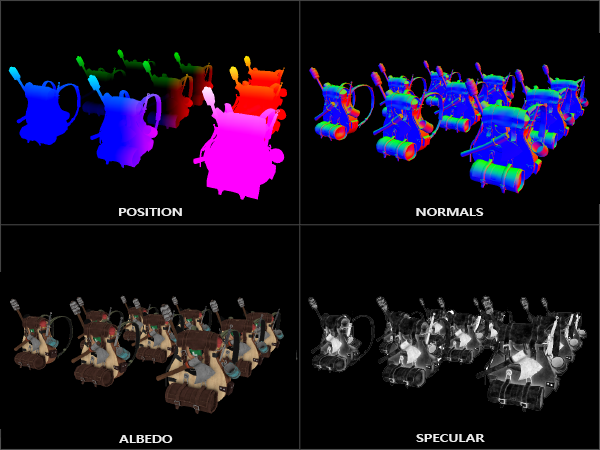
\includegraphics[width=.8\linewidth]{figures/g_buffer_example.png}
   \caption{Esempio di pipeline di deferred rendering da \cite{learnopengl}.}
   \label{fig:deferred-pipeline}
\end{figure}
Il motore sviluppato per questa tesi adotta una pipeline di tipo \emph{deferred}, in quanto offre una base più
flessibile per l’analisi delle prestazioni e per l’integrazione di tecniche di illuminazione avanzate.

\section{Physically Based Rendering (PBR)}
Il \emph{Physically Based Rendering} (PBR) mira a simulare il comportamento reale della luce e dei materiali,
basandosi su modelli fisici dell’interazione tra superfici e radiazione luminosa. A differenza dei modelli
tradizionali, che si affidano spesso a formule empiriche per ottenere un effetto visivamente piacevole, il PBR
definisce le proprietà dei materiali in modo coerente e indipendente dalle condizioni di illuminazione,
garantendo risultati più realistici e prevedibili.
Ogni materiale in un sistema PBR è descritto da un insieme di parametri fisici che ne determinano l’aspetto visivo.
I principali sono:
\begin{itemize}
   \item \textbf{Albedo}: rappresenta il colore base del materiale;
   \item \textbf{Roughness}: controlla la rugosità microscopica della superficie, influenzando la dispersione della luce;
   \item \textbf{Metallic}: indica se il materiale si comporta come un metallo;
   \item \textbf{Normal map}: modifica le normali della superficie per simulare dettagli geometrici fini.
\end{itemize}
Combinando questi parametri, il PBR consente di rappresentare in modo accurato una vasta gamma di materiali,
dai metalli lucidi ai tessuti ruvidi.

\section{Graphics API: OpenGL and Vulkan}
OpenGL e Vulkan rappresentano due approcci concettualmente diversi allo sviluppo di applicazioni grafiche.
OpenGL è un'API di livello alto che semplifica notevolmente la gestione della pipeline grafica: gran parte del lavoro
legato alla sincronizzazione delle risorse, alla gestione della memoria e alla compilazione dei comandi GPU è affidato
al driver. Questo approccio riduce la complessità dello sviluppo, consentendo di ottenere rapidamente risultati visivi,
ma limita il controllo del programmatore sulle prestazioni, soprattutto in scenari con molte luci e geometrie complesse.
OpenGL opera principalmente in modalità single-thread, affidando al driver l’organizzazione dei comandi su GPU, il che può
generare overhead significativi in applicazioni moderne e multithreaded.
Vulkan, al contrario, offre un modello di programmazione a basso livello, dove il programmatore ha il controllo diretto
sulla memoria, sui comandi e sulla sincronizzazione. La pipeline Vulkan richiede la definizione esplicita di tutti i
passaggi di rendering attraverso strutture come \texttt{Render Pass} e \texttt{Command Buffers}, e la gestione della 
sincronizzazione è completamente esplicita mediante \texttt{Semaphore} e \texttt{Fence}. Questo approccio riduce
l’overhead del driver e permette di sfruttare pienamente il multithreading della CPU, rendendo più efficienti
le applicazioni che devono gestire grandi quantità di oggetti e luci in scena. Allo stesso tempo, Vulkan richiede
una conoscenza approfondita dell’architettura hardware e della gestione delle risorse, aumentando la complessità
dello sviluppo rispetto a OpenGL.

\section{Librerie e Strumenti}
Il motore sviluppato utilizza un insieme di librerie open source per la gestione dell’infrastruttura di rendering
e delle funzionalità.
La combinazione di queste librerie ha permesso di ridurre il tempo di sviluppo e concentrarsi sulle differenze
architetturali tra OpenGL e Vulkan.
\begin{itemize}
   \item \textbf{GLFW}: fornisce un’interfaccia multipiattaforma per la creazione di finestre e la gestione dell’input.
      È utilizzata sia per il backend OpenGL che Vulkan;
   \item \textbf{GLAD}: gestisce il caricamento dinamico delle estensioni OpenGL;
   \item \textbf{Vulkan Memory Allocator (VMA)} e \textbf{vk-bootstrap}: semplificano la configurazione e la gestione della memoria
      Vulkan, riducendo la complessità di codice di inizializzazione;
   \item \textbf{glm}: libreria matematica per operazioni su vettori, matrici e trasformazioni 3D;
   \item \textbf{ImGui}: libreria per la costruzione di interfacce grafiche di debug e monitoraggio delle prestazioni in tempo reale;
   \item \textbf{stb\_image}: caricamento di texture in vari formati;
   \item \textbf{ASSIMP}: parsing dei modelli 3D in formato \texttt{.obj} e \texttt{.fbx}.
\end{itemize}

\section{Lavori Correlati}
Diversi studi e progetti hanno analizzato il confronto tra OpenGL e Vulkan, evidenziando vantaggi significativi di
Vulkan in termini di efficienza e parallelismo.
Il \emph{Khronos Group}, nelle specifiche di rilascio e nei documenti ufficiali, evidenzia come Vulkan sia progettata per
minimizzare l’overhead del driver e fornire prestazioni più prevedibili grazie a un controllo esplicito delle risorse e
dell’esecuzione dei comandi \cite{khronos_vulkan_spec,vulkan_overview,google_vulkan_lowoverhead}.
Sul fronte applicativo, motori come \emph{Unreal Engine 5} e \emph{Unity} hanno introdotto backend Vulkan per
ottimizzare la scalabilità su dispositivi moderni, mantenendo al contempo compatibilità con OpenGL su piattaforme legacy.

%----------------------------------------------------------------------------------------
\chapter{Requisiti ed Analisi}
\label{chap:analysis}
%----------------------------------------------------------------------------------------

\section{Requisiti funzionali}

\section{Requisiti non-funzionali}

\section{Constraints}

\section{Evaluation Strategy}

%----------------------------------------------------------------------------------------
\chapter{Design and Architecture}
\label{chap:design}
%----------------------------------------------------------------------------------------

\section{System Overview}

\section{Object-Oriented Design}

\section{Renderer Architecture}

\section{Deferred Rendering Pipeline}

\section{Resource Management}

%----------------------------------------------------------------------------------------
\chapter{Implementation}
\label{chap:implementation}
%----------------------------------------------------------------------------------------

\section{Codebase Structure}

\section{Key Components}

\section{PBR Material System}

\section{Particle Simulation}

\section{Performance GUI}

%----------------------------------------------------------------------------------------
\chapter{Performance Evaluation}
\label{chap:evaluation}
%----------------------------------------------------------------------------------------

\section{Experimental Setup}

\section{Results}

\section{Discussion}

%----------------------------------------------------------------------------------------
\chapterWithoutNumber{Conclusions and Future Work}
\label{chap:conclusions}
%----------------------------------------------------------------------------------------

\paragraph{Summary}

\paragraph{Findings}

\paragraph{Limitations}

\paragraph{Future Work}

% End of thesis
\backmatter

\nocite{*}

\bibliographystyle{alpha}
\bibliography{bibliography}

% TODO: Write acknowledgements (optional)
\begin{acknowledgements}
   Optional. Max 1 page.
\end{acknowledgements}

\end{document}
